\documentclass[12pt]{beamer}
%\includeonlyframes{current}

\mode<presentation>{\usetheme{Warsaw}}
\setbeamertemplate{footline}[frame number]
\usepackage[english]{babel}
\usepackage{times}
\usepackage{url}
\usepackage{graphicx}
\usepackage{hhline}
\usepackage{array}
\usepackage{colortbl}
\usepackage{amsfonts}

\newcommand{\key}[1]{{\color{blue}#1}}
\newcommand{\cmnt}[1]{{\color{gray}#1}}
\newcommand{\str}[1]{{\color{green!50!black}#1}}
\newcommand{\num}[1]{{\color{green!55!blue}#1}}
\newcommand{\defn}[1]{{\color{purple}#1}}
\newcommand{\SC}[1]{\mbox{\sc#1}}
\newcommand{\EM}[1]{\mbox{\em#1}}
\newcommand{\tab}{\hspace{1em}}

\title{Learning from Observations}
\subtitle{Introduction to Artificial Intelligence}
\author{Steven Bethard}
\institute{
  Department of Computer Science\\
  University of Colorado
}
\date{CSCI 3202}


\AtBeginSection[]{
\begin{frame}<beamer>{Outline}
	\tableofcontents[currentsection]
\end{frame}
}

\begin{document}

\begin{frame}
	\titlepage
\end{frame}

\begin{frame}{Outline}
	\tableofcontents
\end{frame}

\section{Learning Basics}
\subsection{Learning Functions}
\begin{frame}{Supervised Learning}
	\begin{block}{Key Ideas}
		\begin{itemize}
			\item Examine pairs of inputs and outputs
			\item Guess a possible function mapping input to output
			\item Predict outputs given new inputs
		\end{itemize}
	\end{block}
	\bigskip
	\begin{columns}
		\begin{column}<2->{1.1in}
			$
			\begin{array}{lll}
			f(1) & = & 1 \\
			f(2) & = & 4 \\
			f(3) & = & 9 \\
			f(4) & = & 16 \\
			f(5) & = & \alt<3->{\alert{25}}{?} \\
			\end{array}
			$
		\end{column}
		\begin{column}<4->{3.1in}
			\begin{tabular}{lll}
			$f$(Romeo and Juliet) & = & Shakespeare \\
			$f$(Tom Sawyer)       & = & Twain \\
			$f$(Macbeth)          & = & Shakespeare \\
			$f$(Huckleberry Finn) & = & Twain \\
			$f$(Othello)          & = & \alt<5->{\alert{Shakespeare}}{?} \\
			\end{tabular}
		\end{column}
	\end{columns}
\end{frame}
\begin{frame}{Supervised Learning Components}
	\begin{block}{Original Function}
		An unknown function $f\!: D_f \rightarrow R_f$
	\end{block}
	\pause
	\begin{block}{Training Examples}
		Pairs of $(x, f(x))$ where $x \in D_f$ and $f(x) \in R_f$
	\end{block}
	\pause
	\begin{block}{Hypothesis Function}
		Some function $h\!: D_f \rightarrow R_f$
	\end{block}
	\pause
	\begin{block}{Learning Goal}
		Pick a hypothesis $h$ as close to $f$ as possible
	\end{block}
\end{frame}
\begin{frame}{Selecting Hypotheses}
	\begin{columns}
		\begin{column}{2.1in}
			Many hypotheses possible:
			
			\bigskip
			\only<1>{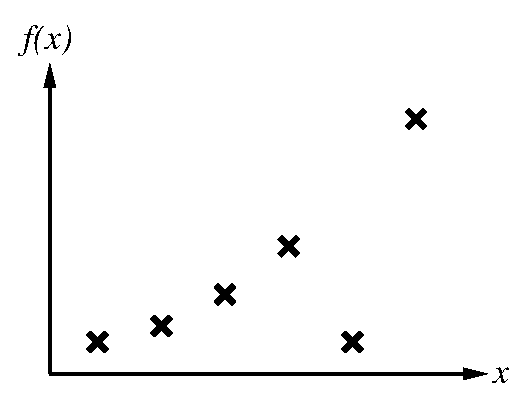
\includegraphics[height=1.5in]{curve-fitting-1}}%
			\only<2>{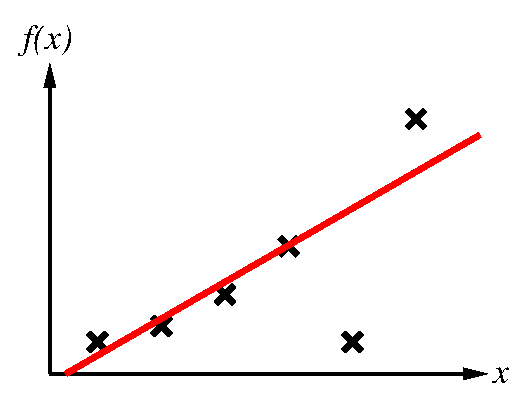
\includegraphics[height=1.5in]{curve-fitting-2}}%
			\only<3>{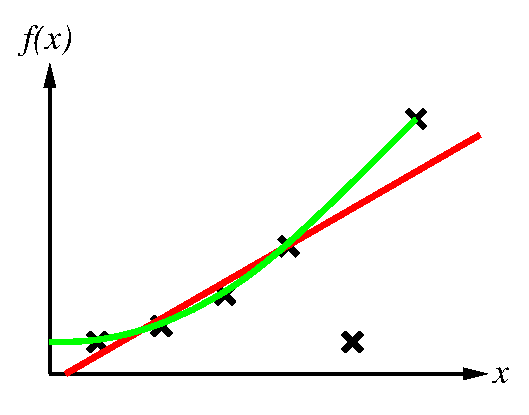
\includegraphics[height=1.5in]{curve-fitting-3}}%
			\only<4>{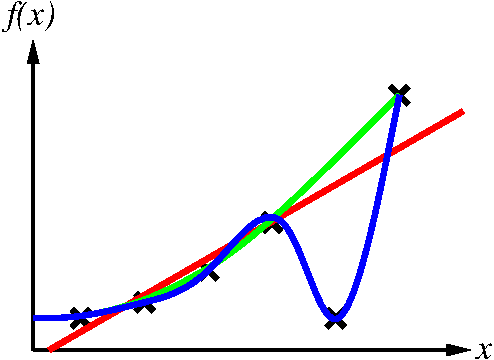
\includegraphics[height=1.5in]{curve-fitting-4}}%
			\only<5->{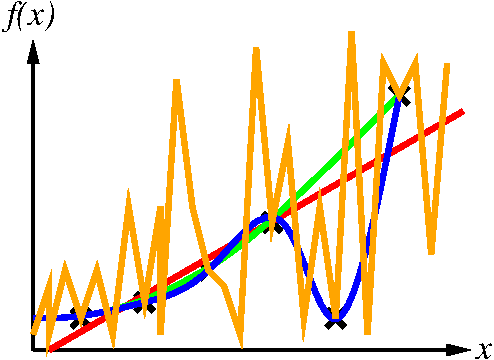
\includegraphics[height=1.5in]{curve-fitting-5}}%
		\end{column}
		\begin{column}<6->{2.1in}
			\begin{block}{Goals}
				\begin{itemize}
					\item Maximize number of examples where $h$ agrees with $f$
					\item Minimize complexity of $h$ function
				\end{itemize}
			\end{block}
			\bigskip
			\uncover<7->{Typically a tradeoff between consistency and simplicity}
		\end{column}
	\end{columns}
\end{frame}
\begin{frame}{Overfitting}
	\begin{block}{Definition}
		A hypothesis $h$ has \alert{overfit} the data if it uses a function that is more complex than necessary to explain the data
	\end{block}
	\smallskip
	\begin{columns}[t]
		\begin{column}<2->{1in}
			Examples: \\
			\medskip
			$
			\begin{array}{lll}
			f(1) & = & 2 \\
			f(2) & = & 4 \\
			f(3) & = & 6 \\
			\end{array}
			$
		\end{column}
		\begin{column}<3->{3in}
			Hypotheses: \\
			\medskip
			$
			\begin{array}{lll}
			h_1(x) & = & 2x \\
			\uncover<4->{h_2(x) & = & \alert<5->{x^3 - 6x^2 + 13x - 6}} \\
			\end{array}
			$ \\
			\medskip
			\uncover<5->{$h_2$ has probably overfit the data} \\
			\uncover<6->{\ldots\ unless $f(x) = x^3 - 6x^2 + 13x - 6$}
		\end{column}
	\end{columns}
	\begin{block}<7->{Lesson}
		Use as many parameters as we expect $f$ to have, no more
	\end{block}
\end{frame}


\subsection{Problem Formulation}
\begin{frame}{Problem Formulation}
	\begin{block}{Defining a Machine Learning Problem}
		Describe the function $f\!: D_f \rightarrow R_f$
		\begin{itemize}
			\item What is $D_f$?
			\item What is $R_f$?
		\end{itemize}
	\end{block}
	\pause
	\begin{columns}
		\begin{column}{2in}
			\begin{block}{Ex: Income Prediction}
				\begin{itemize}
					\pause
					\item $D_f$ = \pause humans
					\pause
					\item $R_f$ = \pause $\mathbb{R}$ (yearly income)
				\end{itemize}
			\end{block}
		\end{column}
		\pause
		\begin{column}{2in}
			\begin{block}{Ex: Cancer Diagnosis}
				\begin{itemize}
					\pause
					\item $D_f$ = \pause animals
					\pause
					\item $R_f$ = \pause $\{\EM{true},\EM{false}\}$
				\end{itemize}
			\end{block}
		\end{column}
	\end{columns}
\end{frame}
\begin{frame}{Decomposing Domain Objects}
	\begin{columns}
		\begin{column}{1.6in}
			Smoker identification: \\
			\smallskip
			\begin{tabular}{lll}
			$f$(John)  & = & \EM{true} \\
			$f$(Mary)  & = & \EM{false} \\
			$f$(Frank) & = & \EM{false} \\
			$f$(Sally) & = & ?
			\end{tabular}
		\end{column}
		\pause
		\begin{column}{2.6in}
			\begin{block}{But name is insufficient!}
				Need to know, e.g.
				\begin{itemize}
					\item smells like cigarettes?
					\item has yellow teeth?
				\end{itemize}
			\end{block}
		\end{column}
	\end{columns}
	\bigskip
	\pause
	\begin{block}{Definition}
		\alert{Attributes} or \alert{features} are the components of a domain object believed to be important for learning the function $f$
	\end{block}
\end{frame}
\begin{frame}{Part of Speech Tagging Example}
	\begin{tabular}{llllll}
		\key{Input}  & \em John & \em broke & \em the & \em red & \em lamp \\
		\pause
		\key{Output} & \sc Noun & \sc Verb  & \sc Det & \sc Adj & \sc Noun \\
	\end{tabular}
	\pause
	\begin{block}{Function Description}
		\begin{itemize}
			\pause
			\item $D_f$ = \pause $\{\EM{a},\EM{aardvark},\EM{abacus},\EM{abalone},\ldots\}$
			\pause
			\item $R_f$ = \pause $\{\SC{Noun},\SC{Verb},\SC{Adj},\SC{Adv},\SC{Det},\ldots\}$
		\end{itemize}
	\end{block}
	\medskip
	\pause
	\begin{columns}
		\begin{column}{2in}
			$f$(\EM{bark}) = \SC{Noun}? \SC{Verb}?
		\end{column}
		\begin{column}{2in}
			\emph{\ldots the \textbf{bark} of the tree \ldots} \\
			\emph{\ldots heard the dog \textbf{bark} \ldots} \\
		\end{column}
	\end{columns}
	\pause
	\begin{block}{Feature Representation}
		$
		\begin{array}{lll}
		f([w_{0}\!=\!\EM{bark}, w_{-1}\!=\!\EM{the}]) & = & \SC{Noun} \\
		f([w_{0}\!=\!\EM{bark}, w_{-1}\!=\!\EM{dog}]) & = & \SC{Verb}
		\end{array}
		$
	\end{block}
\end{frame}
\begin{frame}{Named Entity Recognition Exercise}
	\begin{block}{Definition}
		A \alert{named entity recognition} program find spans of words that are people, locations, organizations, etc.
		
		\medskip
		\begin{tabular}{llllll}
			\key{Input}  & Bill works for Microsoft Corporation\\
			\key{Output} & $[_{\SC{\scriptsize Per}}$ Bill$]$ works for
			               $[_{\SC{\scriptsize Org}}$ Microsoft Corporation$]$ \\
		\end{tabular}
	\end{block}
	\pause
	\begin{block}{Exercise}
		Named entity recognition as supervised learning:
		\begin{itemize}
			\item Describe the function domain
			\item Describe the function range
			\item Describe the feature space
		\end{itemize}
	\end{block}
\end{frame}
\begin{frame}{One Named Entity Recognition Approach}
	\begin{block}{Function Description}
		\begin{itemize}
			\item $D_f$ = \pause $\{\EM{a},\EM{aardvark},\EM{abacus},\EM{abalone},\ldots\}$
			\item $R_f$ = \pause $\{\SC{B-Per},\SC{I-Per},\SC{B-Org},\SC{I-Org},\ldots,\SC{O}\}$
		\end{itemize}
	\end{block}
	\pause
	$
	\begin{array}{lll}
		f(\EM{Bill})        & = & \SC{B-Per} \\
		f(\EM{works})       & = & \SC{O} \\
		f(\EM{for})         & = & \SC{O} \\
		f(\EM{Microsoft})   & = & \SC{B-Org} \\
		f(\EM{Corporation}) & = & \SC{I-Org} \\
	\end{array}
	$
	\pause
	\begin{block}{Typical Features}
		\begin{tabular}{p{1.8in}p{1.8in}}
			Word itself     & Capitalization \\
			Preceding label & First in sentence? \\
		\end{tabular}
	\end{block}
\end{frame}

\subsection{Learning Algorithms}
\begin{frame}{Learning Supervised Models}
	After problem formulation, we apply a \alert{learning algorithm} \\
	\medskip
	\begin{block}{Input}
		A set of $(x, f(x))$ training examples
	\end{block}
	\pause
	\begin{block}{Output}
		A function $h\!: D_f \rightarrow R_f$
	\end{block}
	\pause
	\begin{block}{Goal}
		Pick an $h$ that:
		\begin{itemize}
			\item is consistent with the training examples
			\item does not overfit the data (i.e. is not overly complex)
		\end{itemize}
	\end{block}
\end{frame}
\begin{frame}{Evaluating Learning Algorithms}
	\begin{enumerate}
		\item Train learning algorithm on examples $E_{\EM{\scriptsize train}}$
		\item Learning algorithm produces a hypothesis $h$
		\item Test hypothesis on new examples $E_{\EM{\scriptsize test}}$ \uncover<2->{- \alert{Don't peek!}}
	\end{enumerate}
	\begin{columns}
		\begin{column}<3->{2in}
			Train:
			$
			\begin{array}[t]{ll|l}
				F_1 & F_2 & \EM{Class} \\
				\hline
				0   & a   & \EM{true} \\
				0   & b   & \EM{false} \\
				0   & c   & \EM{false} \\
				1   & b   & \EM{false} \\
			\end{array}
			$
		\end{column}
		\begin{column}<6->{2in}
			Test:
			$
			\begin{array}[t]{ll|l}
				F_1 & F_2 & \EM{Class} \\
				\hline
				1   & a   & \EM{true} \\
				0   & b   & \EM{false} \\
				0   & c   & \EM{false} \\
				1   & c   & \EM{true} \\
			\end{array}
			$
		\end{column}
	\end{columns}
	\begin{columns}
		\begin{column}<4->{2in}
			\begin{block}{Algorithm 1}
				Always classify as \EM{false}
				\\
				\uncover<7->{\tab Performance:} \uncover<8->{$\frac{2}{4} = 0.5$}
			\end{block}
		\end{column}
		\begin{column}<5->{2in}
			\begin{block}{Algorithm 2}
				If $a$ then \EM{true}, else \EM{false}
				\\
				\uncover<7->{\tab Performance:} \uncover<9->{$\frac{3}{4} = 0.75$}
			\end{block}
		\end{column}
	\end{columns}
\end{frame}
\begin{frame}{Learning Curves}
	\begin{itemize}
		\item Train on increasing fractions of training data
		\item Test each of the resulting hypotheses on the test data
	\end{itemize}
	\pause
	\begin{center}
		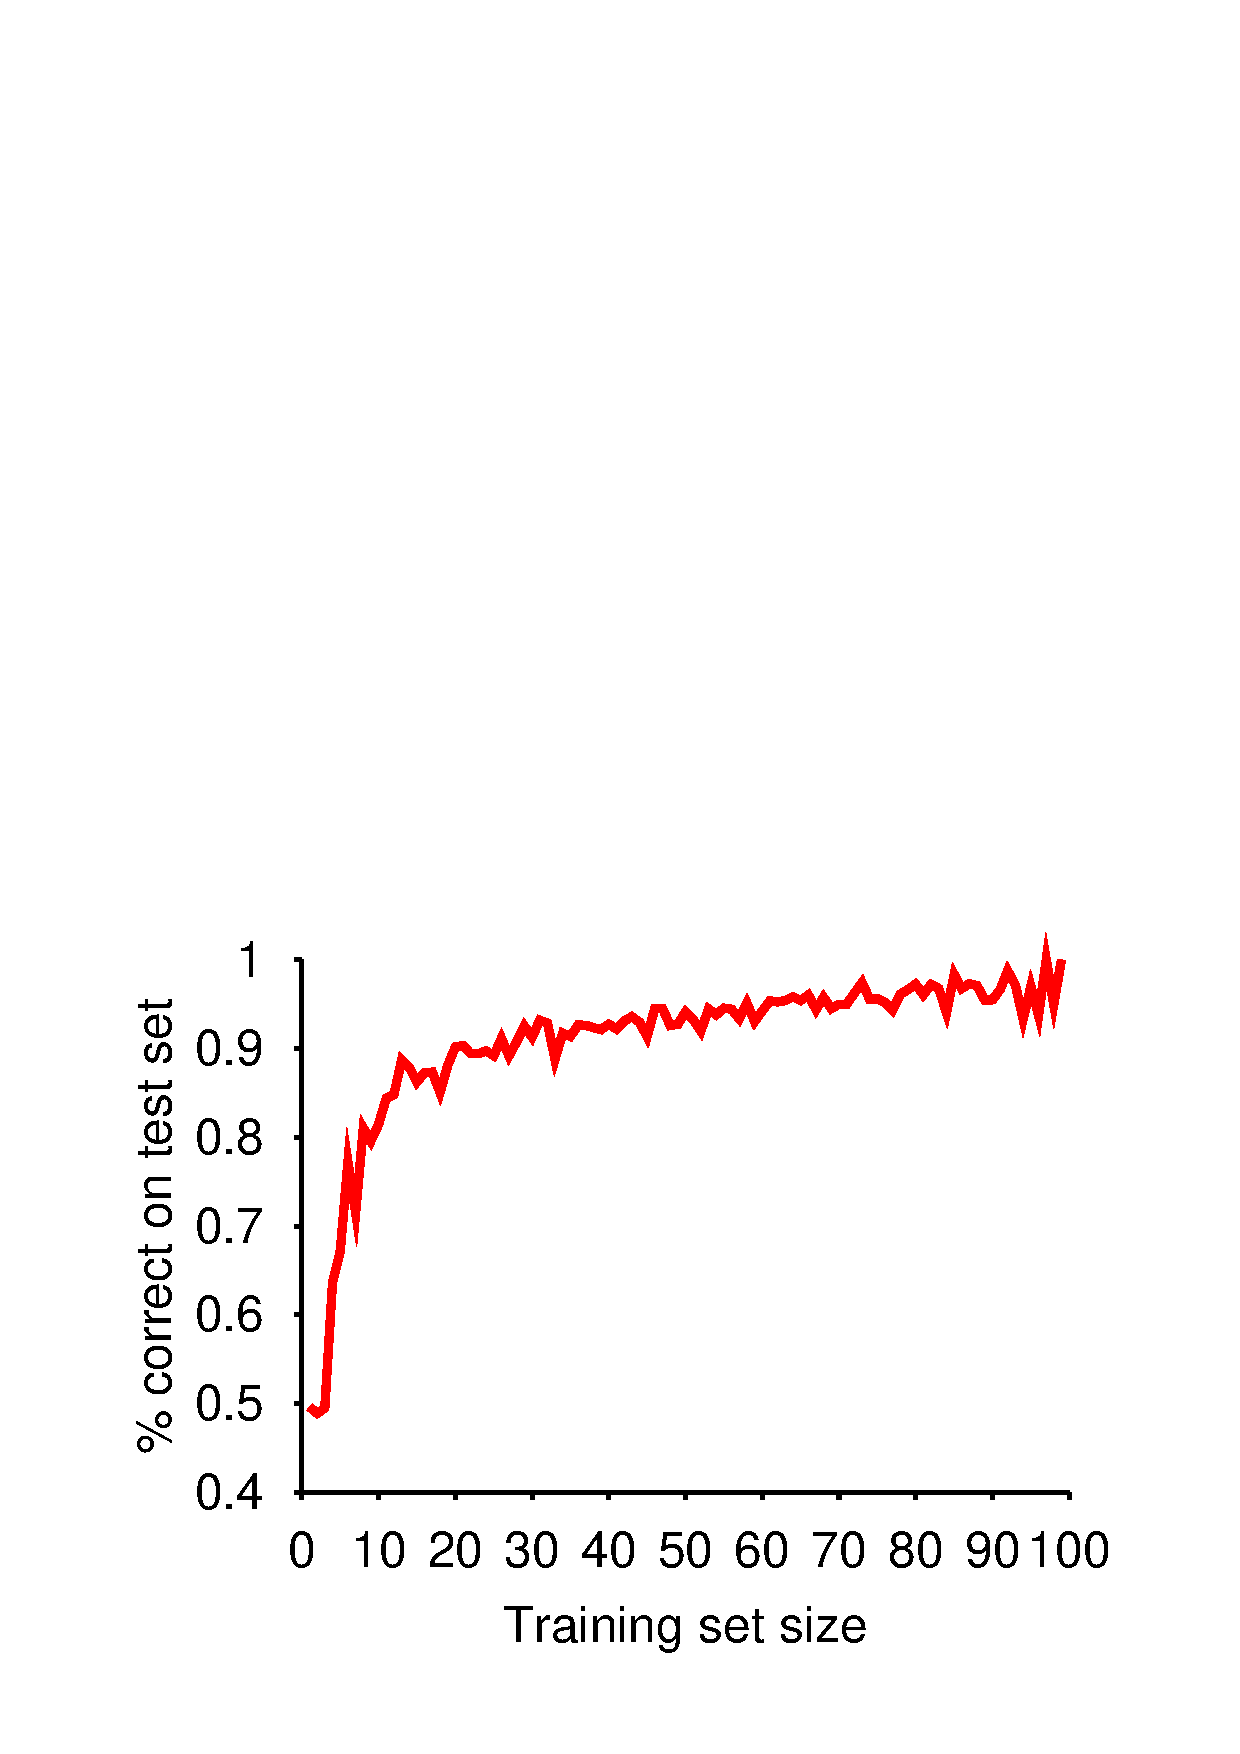
\includegraphics[height=2in]{restaurant-dtl-curve}
	\end{center}
\end{frame}


\section{Decision Trees}
\subsection{Decision Tree Basics}
\begin{frame}{Decision Trees}
	\begin{columns}
		\begin{column}{2.7in}
			\centering
			Should I play golf today? \\
			\bigskip
			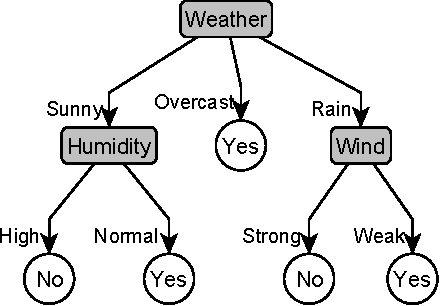
\includegraphics[width=2.7in]{play_golf}
		\end{column}
		\begin{column}{1.5in}
			\begin{block}{Function}
				$D_f$ = days
				
				$R_f$ = $\{\EM{Yes}, \EM{No}\}$
			\end{block}
			\bigskip
			\begin{block}{Features}
				\begin{itemize}
					\item Weather
					\item Humidity
					\item Wind
				\end{itemize}
			\end{block}
		\end{column}
	\end{columns}
\end{frame}
\begin{frame}{Decision Trees as Functions}
	\begin{columns}[t]
		\begin{column}{2in}
			$f(X, Y) = X \EM{ xor } Y$ \\[1em]
			\includegraphics[scale=.75]{xor}
		\end{column}
		\begin{column}{2in}
			$f(A, B, C) = (A \land B) \lor \lnot C$ \\[1em]
			\includegraphics[scale=.75]{abc}
		\end{column}
	\end{columns}
\end{frame}


\subsection{Decision Tree Learning}
\begin{frame}{Learning Decision Trees}
	\begin{enumerate}
		\item Select a feature $F$ for the node
		\item For each value of $F$, create a child node
		\item Sort training examples into child nodes
		\item If examples are sorted perfectly, terminate
		\item Else, repeat the process for each child node
	\end{enumerate}
	\begin{columns}
		\begin{column}<2->{1.7in}
			$
			\begin{array}{cc|c}
				X          &  Y          & f(X, Y) \\
				\hline
				\EM{true}  & \EM{true}   & \EM{true} \\
				\EM{true}  & \EM{false}  & \EM{false} \\
				\EM{false} & \EM{true}   & \EM{true} \\
				\EM{false} & \EM{false}  & \EM{true} \\
			\end{array}
			$
		\end{column}
		\begin{column}{2.6in}
			\only<-2>{\invisible{\includegraphics[scale=.75]{impl}}}%
			\only<3>{\includegraphics[scale=.75]{impl-1}}%
			\only<4>{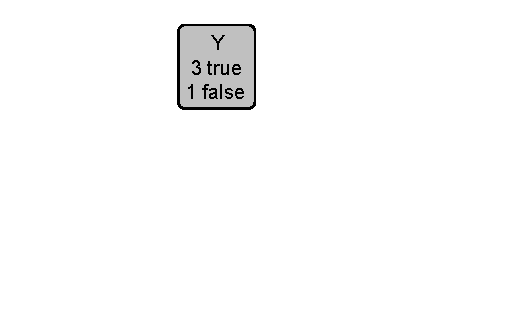
\includegraphics[scale=.75]{impl-2}}%
			\only<5>{\includegraphics[scale=.75]{impl-3}}%
			\only<6>{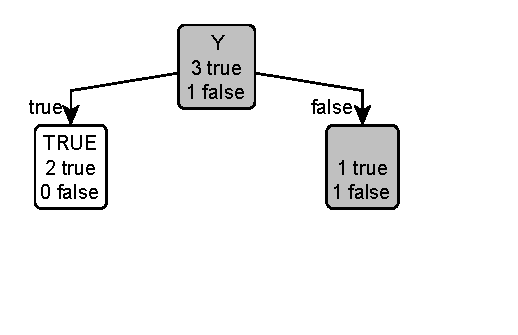
\includegraphics[scale=.75]{impl-4}}%
			\only<7>{\includegraphics[scale=.75]{impl-5}}%
			\only<8>{\includegraphics[scale=.75]{impl-6}}%
			\only<9>{\includegraphics[scale=.75]{impl-7}}%
		\end{column}
	\end{columns}
\end{frame}
\begin{frame}[label=decision-tree-exercise]{Decision Tree Exercise}
	\begin{columns}
		\begin{column}{1.8in}
			Build a decision tree for: \\
			\bigskip
			$
			\begin{array}{ll|l}
				F_1 & F_2 & \EM{Class} \\
				\hline
				0   & a   & \EM{true} \\
				0   & b   & \EM{false} \\
				1   & c   & \EM{true} \\
				0   & c   & \EM{false} \\
				1   & b   & \EM{false} \\
				1   & a   & \EM{true} \\
			\end{array}
			$
		\end{column}
		\pause
		\begin{column}{1.8in}
			Two possible solutions:
		
			\centering
			\bigskip
			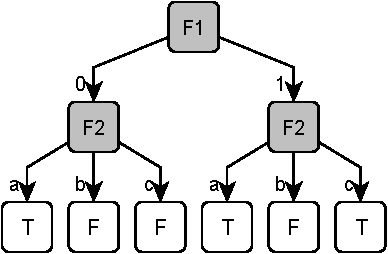
\includegraphics[scale=.6]{exercise-1}
			
			\bigskip
			\includegraphics[scale=.6]{exercise-2}
		\end{column}
	\end{columns}
\end{frame}


\subsection{Features and Information}
\begin{frame}{Selecting Features for Decision Trees}
	\begin{block}{Feature Selection Order}
		\begin{itemize}
			\item Different orders result in different trees
			\item ``Good'' features should be used before ``poor'' ones
		\end{itemize}
	\end{block}
	\pause
	\begin{block}{What is a ``good'' feature?}
		One whose values predict the class labels \\
	\end{block}
	\pause
	\medskip
	\begin{columns}
		\begin{column}{1.2in}
			$
			\begin{array}{lll}
			F_1 & F_2 & \EM{Class} \\
			\hline
			a & 0 & \EM{true} \\
			a & 1 & \EM{true} \\
			b & 0 & \EM{false} \\
			b & 1 & \EM{false} \\
			\end{array}
			$
		\end{column}
		\pause
		\begin{column}{1.8in}
			$F_1$ is a \alert{good} feature \\
			\bigskip
			$F_2$ is a \alert{poor} feature
		\end{column}
	\end{columns}
\end{frame}
\begin{frame}{Information}
	\begin{block}{Good features provide more information}
		Information can be quantified in terms of bits
	\end{block}
	\pause
	Task: Encode \texttt{abacabad} using as few bits as possible
	\pause
	\medskip
	\begin{columns}[t]
		\begin{column}{1.8in}
			Simple Encoding:
			\begin{tabular}{ll}
				a & 00 \\
				b & 01 \\
				c & 10 \\
				d & 11 \\
			\end{tabular} \\
			\pause
			\medskip
			\texttt{abacabad} $\rightarrow$ 16 bits \texttt{0001001000010011}
		\end{column}
		\pause
		\begin{column}{1.8in}
			Using Probability:
			\begin{tabular}{ll}
			a & 0 \\
			b & 10 \\
			c & 110 \\
			d & 111 \\
			\end{tabular} \\
			\pause
			\medskip
			\texttt{abacabad} $\rightarrow$ 14 bits \texttt{01001100100111}
		\end{column}
	\end{columns}
	\pause
	\bigskip
	\alert{More likely values can be encoded in fewer bits!}
\end{frame}
\begin{frame}{Entropy}
	\begin{block}{Definition}
		The \alert{entropy} of a random variable $X$ is: \\
		\smallskip
		\tab\tab$H(X) = -\sum\limits_{x \in X}P(x)\log_2 P(x)$
	\end{block}
	\pause
	\begin{block}{Bit-based Interpretation}
		Smallest number of bits that can encode a stream of values from $X$'s distribution
	\end{block}
	\pause
	\begin{block}{Intuitions}
		\begin{itemize}
			\item High entropy $\rightarrow$ boring (e.g. uniform) distribution
			\item Low entropy $\rightarrow$ interesting distribution
		\end{itemize}
	\end{block}
\end{frame}
\begin{frame}{Entropy}
	\begin{columns}
		\begin{column}{1.1in}
			\begin{tabular}{ll}
				X       & Y   \\
				\hline
				math    & yes \\
				history & no  \\
				cs      & yes \\
				math    & no  \\
				math    & no  \\
				cs      & yes \\
				history & no  \\
				math    & yes \\
			\end{tabular}
		\end{column}
		\begin{column}{3.1in}
			\pause
			$
			\extrarowheight=2pt
			\begin{array}{lll}
				H(X)        & = & \pause -\sum\limits_{x \in X}P(x)\log_2 P(x) \\
				     \pause & = & -P(\EM{math})\log_2 P(\EM{math}) \\
				            &   & -P(\EM{history})\log_2 P(\EM{history}) \\
				            &   & -P(\EM{cs})\log_2 P(\EM{cs}) \\
				     \pause & = & -\frac{1}{2}\log_2\frac{1}{2} 
				                  -\frac{1}{4}\log_2\frac{1}{4}
				                  -\frac{1}{4}\log_2\frac{1}{4} \\
				     \pause & = & -\frac{1}{2}(-1) - \frac{1}{4}(-2) - \frac{1}{4}(-2) \\
				     \pause & = & \frac{1}{2} + \frac{1}{2} + \frac{1}{2} \\
				     \pause & = & 1.5 \\
				\\
				\pause
				H(Y)        & = & \pause 1.0 \\
			\end{array}
			$
		\end{column}
	\end{columns}
\end{frame}
\begin{frame}{Specific Conditional Entropy}
	\begin{columns}
		\begin{column}{1.1in}
			\begin{tabular}{ll}
				X               & Y   \\
				\hline
				math            & yes \\
				history         & no  \\
				\alert<4-5>{cs} & \alert<4>{yes} \\
				math            & no  \\
				math            & no  \\
				\alert<4-5>{cs} & \alert<4>{yes} \\
				history         & no  \\
				math            & yes \\
			\end{tabular}
		\end{column}
		\begin{column}{3.1in}
			\begin{block}{Specific Conditional Entropy}
				$H(Y|X\!=\!x) = -\sum\limits_{y \in Y}P(y|x)\log_2 P(y|x)$
			\end{block}
			\small
			$
			\extrarowheight=2pt
			\begin{array}{@{}l@{}l@{}l@{}}
				\uncover<2->{H(Y|X\!=\!\EM{cs})}
				& \uncover<2->{=}
				& \uncover<3->{\alert<4>{-P(\EM{yes}|\EM{cs})\log_2 P(\EM{yes}|\EM{cs})}}
				\\
				&
				& \uncover<3->{\alert<5>{-P(\EM{no}|\EM{cs})\log_2 P(\EM{no}|\EM{cs})}}
				\\
				& \uncover<4->{=}
				& \uncover<4->{\alert<4>{-1 \log_2 1}}\uncover<5->{\alert<5>{-0 \log_2 0}}
				\\
				& \uncover<6->{=}
				& \uncover<6->{-1 \cdot 0 - 0 \cdot \infty}
				\\
				& \uncover<7->{=}
				& \uncover<7->{0} \\
			\end{array}
			$ \\
			\medskip
			\uncover<8->{In other words, $X\!=\!\EM{cs}$ is a great predictor of $Y$}
		\end{column}
	\end{columns}
\end{frame}
\begin{frame}{Conditional Entropy}
	\begin{columns}
		\begin{column}{1.1in}
			\begin{tabular}{ll}
				X               & Y   \\
				\hline
				math            & yes \\
				history         & no  \\
				cs              & yes \\
				math            & no  \\
				math            & no  \\
				cs              & yes \\
				history         & no  \\
				math            & yes \\
			\end{tabular}
		\end{column}
		\begin{column}{3.1in}
			\begin{block}{Conditional Entropy}
				$
				\begin{array}{lll}
					H(Y|X) & = & \sum\limits_{x \in X}P(X\!=\!x)H(Y|X\!=\!x)
				\end{array}
				$
			\end{block}
			\pause
			\small
			Given:
			$
			\begin{array}[t]{lll}
			H(Y|X\!=\!\EM{math})    & = & 1 \\
			H(Y|X\!=\!\EM{history}) & = & 0 \\
			H(Y|X\!=\!\EM{cs})      & = & 0 \\
			\end{array}
			$ \\
			\smallskip
			\pause
			$
			\extrarowheight=2pt
			\begin{array}{@{}l@{\hspace{2pt}}l@{\hspace{2pt}}l@{}}
				H(Y|X) & = & \pause P(X\!=\!\EM{math}) H(Y|X\!=\!\EM{math}) + \mbox{}\\
				       &   & P(X\!=\!\EM{history}) H(Y|X\!=\!\EM{history}) + \mbox{}\\
				       &   & P(X\!=\!\EM{cs}) H(Y|X\!=\!\EM{cs}) \\
				\pause & = & \frac{1}{2} \cdot 1 + \frac{1}{4} \cdot 0 + \frac{1}{4} \cdot 0 \pause = \frac{1}{2}\\
				
			\end{array}
			$ \\
			\medskip
			\pause
			In other words, $X$ is a good predictor of $Y$
		\end{column}
	\end{columns}
\end{frame}
\begin{frame}{Information Gain}
	\begin{columns}
		\begin{column}{1.1in}
			\begin{tabular}{ll}
				X               & Y   \\
				\hline
				math            & yes \\
				history         & no  \\
				cs              & yes \\
				math            & no  \\
				math            & no  \\
				cs              & yes \\
				history         & no  \\
				math            & yes \\
			\end{tabular}
		\end{column}
		\begin{column}{3.1in}
			\begin{block}{Information Gain}
				$IG(Y|X) = H(Y) - H(Y|X)$
			\end{block}
			\pause
			\begin{block}{Intuitive Explanation}
				How many bits would it save to know $X$?
			\end{block}
			\pause
			$
			\begin{array}[t]{lll}
			H(Y|X)  & = & 0.5 \\
			H(Y)    & = & 1 \\
			\\
			\pause
			IG(Y|X) & = & \pause 1 - 0.5 = 0.5
			\end{array}
			$
		\end{column}
	\end{columns}
\end{frame}
\begin{frame}{Decision Trees and Information Gain}
	\textbf{\key{Select the feature with the highest information gain}}
	\pause
	\medskip
	\begin{columns}[T]
		\begin{column}{0.6in}
			\small
			$
			\begin{array}{@{}l@{\hspace{2pt}}l@{\hspace{2pt}}|@{\hspace{2pt}}l@{}}
				F_1 & F_2 & Y \\
				\hline
				0   & a   & \SC{t} \\
				0   & b   & \SC{f} \\
				1   & c   & \SC{t} \\
				0   & c   & \SC{f} \\
				1   & b   & \SC{f} \\
				1   & a   & \SC{t} \\
			\end{array}
			$
		\end{column}
		\pause
		\begin{column}{3.8in}
			\small
			$
			\extrarowheight=2pt
			\begin{array}{@{}l@{\hspace{2pt}}l@{\hspace{2pt}}l@{}}
				H(Y)               & = & \pause -P(\SC{t})\log_2 P(\SC{t}) - P(\SC{f})\log_2 P(\SC{f}) \\
				\pause
				                   & = & -\frac{1}{2}\log_2 \frac{1}{2} - \frac{1}{2}\log_2 \frac{1}{2} \pause = 1 \\
				\pause
				H(Y|F_1\!\!=\!\!0) & = & \pause -P(\SC{t}|0)\log_2 P(\SC{t}|0) - \pause P(\SC{f}|0)\log_2 P(\SC{f}|0) \\
				\pause
				                   & = & - \frac{1}{3}\log_2 \frac{1}{3} - \pause \frac{2}{3}\log_2 \frac{2}{3} \pause = 0.92\\
				\pause         
				H(Y|F_1\!\!=\!\!1) & = & \pause \ldots = 0.92\\
				\pause         
				H(Y|F_1)           & = & \pause P(F_1\!\!=\!\!0) H(Y|F_1\!\!=\!\!0) + P(F_1\!\!=\!\!1) H(Y|F_1\!\!=\!\!1) \\
				\pause         
				                   & = & 0.5 \cdot 0.92 + \pause 0.5 \cdot 0.92 \pause = 0.92 \\
				\pause
				IG(Y|F_1)          & = & \pause H(Y) - H(Y|F_1) \pause = 1 - 0.92 \pause = 0.08 \\
				\pause         
				IG(Y|F_2)          & = & \pause \mbox{\alert{ Your turn! }} \pause = 0.67 \\
			\end{array}
			$ \\
			\medskip
			\pause
			So $F_2$ is a much better feature to split on \hyperlink{decision-tree-exercise<2>}{\beamerbutton{See Example}}
		\end{column}
	\end{columns}
\end{frame}


\section{Ensemble Learning}
\begin{frame}{Ensemble Learning}
	\begin{block}{Key Idea}
		Two (or more) classifiers are better than one
	\end{block}
	\begin{center}
		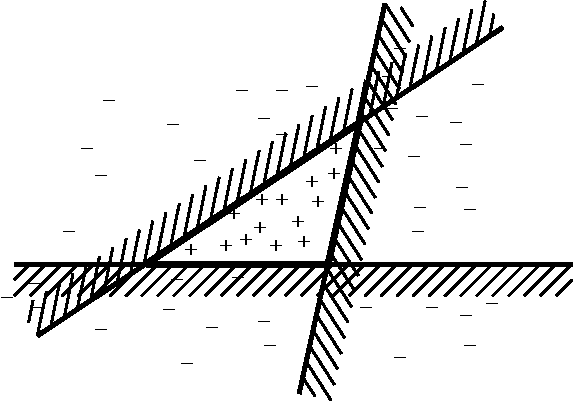
\includegraphics[height=1.8in]{ensemble-expressiveness}
	\end{center}
\end{frame}


\subsection{Bagging}
\begin{frame}[<+->]{Bagging}
	\begin{block}{Key Ideas}
		\begin{itemize}
			\item Error is partly due to particular choice of training set
			\item Create $m$ similar training sets and learn $m$ models
		\end{itemize}
	\end{block}
	\begin{block}{Bagging (\textbf{B}ootstrap \textbf{agg}regat\textbf{ing})}
		Given a training set of $n$ examples:
		\begin{enumerate}
			\item Generate $m$ new training sets (\alert{bootstrap samples})
				\begin{itemize}
					\item Each new training set contains $n$ examples
					\item Examples selected randomly, with replacement
				\end{itemize}
			\item Train $m$ models on the $m$ new training sets
			\item Classify new examples by taking the majority vote
		\end{enumerate}
	\end{block}
\end{frame}
\begin{frame}{Bagging Exercise}
	\begin{columns}
		\begin{column}{2.8in}
			\begin{itemize}
				\item Generate two bootstrap samples
				\item Use indices $[1, 3, 2, 3]$ $[2, 0, 3, 2]$
				\item Create a decision tree for each
				\item Classify $000$ and $101$
			\end{itemize}
		\end{column}
		\begin{column}{1.2in}
			$
			\begin{array}{lll|l}
				F_1 & F_2 & F_3 & C \\
				\hline
				0   & 1   & 1   & T \\
				0   & 1   & 0   & F \\
				0   & 0   & 1   & F \\
				1   & 1   & 0   & T
			\end{array}
			$
		\end{column}
	\end{columns}
	\pause
	\begin{columns}
		\begin{column}{2in}
			\begin{block}{Sample 1}
				$
				\begin{array}{lll|l}
					0   & 1   & 0   & F \\
					1   & 1   & 0   & T \\
					0   & 0   & 1   & F \\
					1   & 1   & 0   & T
				\end{array}
				$
				\begin{tabular}{l}
					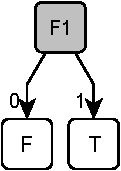
\includegraphics[height=.8in]{bagging-1}
				\end{tabular}
			\end{block}
		\end{column}
		\begin{column}{2in}
			\begin{block}{Sample 2}
				$
				\begin{array}{lll|l}
					0   & 0   & 1   & F \\
					0   & 1   & 1   & T \\
					1   & 1   & 0   & T \\
					0   & 0   & 1   & F
				\end{array}
				$
				\begin{tabular}{l}
					\includegraphics[height=.8in]{bagging-2}
				\end{tabular}
			\end{block}
		\end{column}
	\end{columns}
	\begin{center}
		$
		\begin{array}{lllll}
			\EM{classify}(000) & = & \EM{majority}([F, F]) & = & F \\
			\EM{classify}(101) & = & \EM{majority}([T, F]) & = & ?
		\end{array}
		$
	\end{center}
\end{frame}
\begin{frame}{Bagging Behavior}
	\begin{center}
		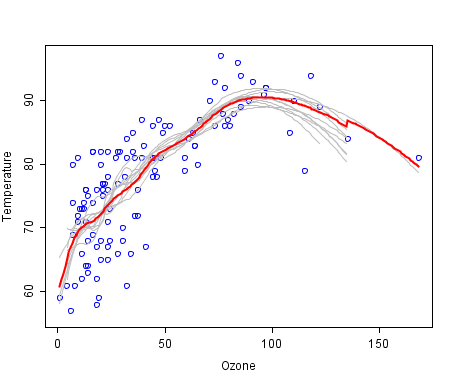
\includegraphics[scale=0.5]{ozone}
	\end{center}
\end{frame}
\begin{frame}{Bagging Properties}
	\begin{block}{Complexity}
		\begin{itemize}
			\pause
			\item Training time: \pause $m$ times original
			\pause
			\item Model size: \pause $m$ times original
			\pause
			\item Classification time: \pause $m$ times original
		\end{itemize}
	\end{block}
	\pause
	\begin{block}{Practical Issues}
		\begin{itemize}
			\item Can improve performance of unstable learners
			\item Typically does not improve stable learners
		\end{itemize}
	\end{block}
\end{frame}

\subsection{Boosting}
\begin{frame}[<+->]{Boosting}
	\begin{block}{Key Ideas}
		\begin{itemize}
			\item Look at examples the first classifier got wrong
			\item Create new models that do better on these
		\end{itemize}
	\end{block}
	\begin{block}{Boosting}
		\begin{enumerate}
			\item Start with all training samples weighted equally
			\item\label{train-step} Train a model (e.g. a single feature \alert{decision stump})
			\item\label{weight-step} Increase the weight of all misclassified examples
			\item Repeat steps \ref{train-step} and \ref{weight-step} until $m$ models are generated
		\end{enumerate}
	\end{block}
\end{frame}
\begin{frame}{Boosting Example}
	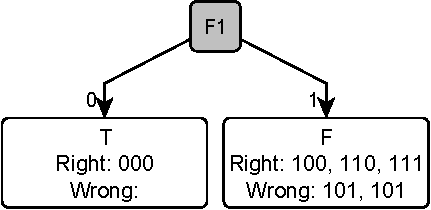
\includegraphics[width=1.4in]{boosting_f1}
	\includegraphics[width=1.4in]{boosting_f2}
	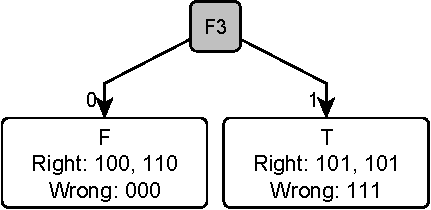
\includegraphics[width=1.4in]{boosting_f3}
	\medskip
	\small
	\begin{columns}
		\begin{column}{1.5in}
			$
			\begin{array}{@{}lll|l|l@{}}
				F_1 & F_2 & F_3 & C & W \\
				\hline
				0 & 0 & 0 & T & 1 \\
				1 & 0 & 0 & F & \alt<5->{\alert<5>{5}}{1} \\
				1 & 1 & 0 & F & 1 \\
				1 & 0 & 1 & T & \alt<9->{\alert<9>{4}}{1} \\
				1 & 0 & 1 & T & \alt<9->{\alert<9>{4}}{1} \\
				1 & 1 & 1 & F & 1 \\
			\end{array}
			$
		\end{column}
		\begin{column}{2.3in}
			\uncover<2->{$
			\begin{array}{@{}lll@{}}
				F_1 \rightarrow \uncover<3->{\frac{4}{6}}
				&
				F_2 \rightarrow \uncover<3->{\frac{5}{6}}
				&
				F_3 \rightarrow \uncover<3->{\frac{4}{6}}
			\end{array}
			$} \\
			\uncover<4->{Select $F_2$ model, update weights} \\
			\medskip
			\uncover<6->{$
			\begin{array}{@{}lll@{}}
				F_1 \rightarrow \uncover<7->{\frac{8}{10}}
				&
				F_2 \rightarrow \uncover<7->{\frac{5}{10}}
				&
				F_3 \rightarrow \uncover<7->{\frac{8}{10}}
			\end{array}
			$} \\
			\uncover<8->{Select $F_1$ model, update weights} \\
			\medskip
			\uncover<10->{$
			\begin{array}{@{}lll@{}}
				F_1 \rightarrow \uncover<11->{\frac{8}{16}}
				&
				F_2 \rightarrow \uncover<11->{\frac{11}{16}}
				&
				F_3 \rightarrow \uncover<11->{\frac{14}{16}}
			\end{array}
			$} \\
			\uncover<12->{Select $F_3$ model} \\
		\end{column}
	\end{columns}
	\medskip
	\uncover<13->{Classification by voting:}
	\uncover<14->{$\frac{1}{4} \cdot \EM{model}_{F_1} + \frac{1}{5} \cdot \EM{model}_{F_2} + \frac{1}{7} \cdot \EM{model}_{F_3}$}
	\\
	\uncover<15->{Classifying the example $100$:}
	\uncover<16->{
	$
	\frac{1}{4} \cdot \alt<17->{F}{?} +
	\frac{1}{5} \cdot \alt<17->{T}{?} +
	\frac{1}{7} \cdot \alt<17->{F}{?}
	$}\uncover<18->{, so $F$}
\end{frame}
\begin{frame}{Boosting Properties}
	\begin{block}{Complexity}
		\begin{itemize}
			\item Training time: \uncover<2->{$m$ times original}
			\item Model size: \uncover<2->{$m$ times original}
			\item Classification time: \uncover<2->{$m$ times original}
		\end{itemize}
		\uncover<3->{Usually acceptable when using e.g. decision stumps}
	\end{block}
	\begin{block}<4->{Theoretical Properties}
		\begin{itemize}
			\item With a large enough $m$, produces a perfect classifier
			\item<5-> In practice, $m$ is selected through experimentation
		\end{itemize}
	\end{block}
\end{frame}

\subsection{Random Forests}
\begin{frame}[<+->]{Random Forests}
	\begin{block}{Key Ideas}
		\begin{itemize}
			\item Voting works better when classifiers are independent
			\item Partially random trees should be more independent
		\end{itemize}
	\end{block}
	\begin{block}{Random Forests}
		\begin{enumerate}
			\item\label{sample-step} Generate a bootstrap sample of $n$ examples
			\item\label{select-step} For each node, select $k$ features at random
			\item\label{split-step} Split on the feature with the highest information gain
			\item Repeat steps \ref{sample-step}, \ref{select-step} and \ref{split-step} to generate $n$ decision trees
			\item Classify by taking the majority vote
		\end{enumerate}
	\end{block}
\end{frame}
\begin{frame}{Random Forest Exercise}
	\begin{columns}
		\begin{column}{1.2in}
			\small
			$
			\begin{array}{lll|l}
				F_0 & F_1 & F_2 & C \\
				\hline
				0   & 0   & 0   & F \\
				0   & 0   & 1   & F \\
				0   & 1   & 1   & F \\
				1   & 0   & 1   & F \\
				1   & 0   & 0   & T \\
				1   & 1   & 1   & T \\
			\end{array}
			$
		\end{column}
		\begin{column}{2.8in}
			\begin{itemize}
				\item Generate a bootstrap sample
				\item Example indices $[0, 5, 0, 1, 5, 4]$
				\item Generate a random decision tree
				\item Feature indices $[1, 2]$ then $[2, 0]$
			\end{itemize}
		\end{column}
	\end{columns}
	\pause
	\begin{columns}
		\begin{column}{1.2in}
			\small
			$
			\begin{array}{lll|l}
				F_0 & F_1 & F_2 & C \\
				\hline
				0   & 0   & 0   & F \\
				1   & 1   & 1   & T \\
				0   & 0   & 0   & F \\
				0   & 0   & 1   & F \\
				1   & 1   & 1   & T \\
				1   & 0   & 0   & T \\
			\end{array}
			$
		\end{column}
		\begin{column}{2.8in}
			\includegraphics[width=2in]{random-tree}
		\end{column}
	\end{columns}
\end{frame}
\begin{frame}[<+->]{Random Forest Properties}
	\begin{block}{Disadvantages}
		\begin{itemize}
			\item Hard to estimate complexity due to random factor
			\item $k$ (\# of features) must be determined experimentally
		\end{itemize}
	\end{block}
	\begin{block}{Advantages}
		\begin{itemize}
			\item State of the art performance on many datasets
			\item Relatively simple to implement
			\item Expected error can be determined while training
				\begin{itemize}
					\item Bootstrap sample leaves out about $\frac{1}{3}$ of examples
					\item Use these out-of-bag examples to test individual trees
					\item Collect votes from all trees to get overall accuracy
				\end{itemize}
		\end{itemize}
	\end{block}
\end{frame}

\part{Key Ideas}
\begin{frame}{Key Ideas}
	\begin{block}{Supervised Learning}
		\begin{itemize}
			\item Input: $(x, f(x))$ examples
			\item Output: $h$, a guess at $f$
			\item Domain objects usually decomposed into features
		\end{itemize}
	\end{block}
	\begin{block}{Decision Trees}
		\begin{itemize}
			\item Each node splits examples by feature values
			\item Best feature yields the highest information gain
			\item Bagging, boosting and random forests combine trees
		\end{itemize}
	\end{block}
\end{frame}

\end{document}


